% !TeX root = ../main.tex

\section{Nonlinear equations}

$f$, we want to find $\alpha\in\mathbb{R}$ zero of $f$ such that $f(\alpha)=0$

It is not easy to find the zero of a function when
$\mathbb{P}_n\,\,n>4$. From here we need to approximate the zeros of a nonlinear function.

An example of physical phenomenol: the ideal gas equation:
$$pV=nRT$$
To find $V$
$$\left[
    p+a\left(
        \frac{N}{V}
    \right)^2
\right](V-Nb)=kNT$$
A nonlinear equation, although we know the pressure, the temperature and the constants $a$ and $k$, it is not easy to solve.

We use \textbf{iterative methods}
$$\underlabel{x^{(0)}}{Initial guess}$$

\begin{figure}[!ht]
    \begin{minipage}{\linewidth}
        \centering
        \makebox[\textwidth][c]{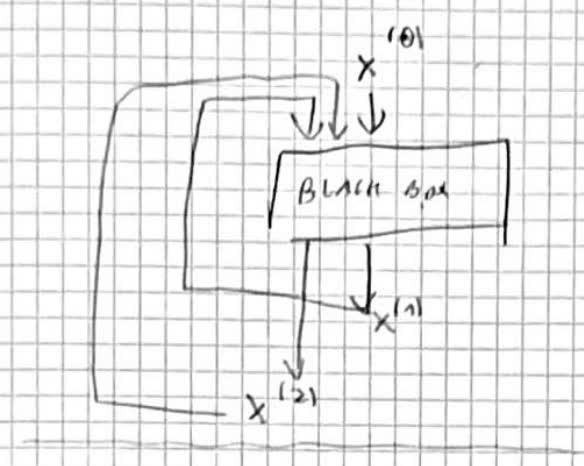
\includegraphics[width=0.5\textwidth]{images/Screenshot from 2022-09-20 22-39-23.png}}%
        %\caption{Black box}
        %\label{BarsNielsenCrop}
    \end{minipage}
\end{figure}

$$x^{(k)}\simeq\alpha$$
Ideally I want
$$\lim_{k\rightarrow\infty}x^{(k)}=\alpha$$
\textbf{Convergence}, or equivalently
$$e^{(k)}=\alpha-x^{(k)}$$
$$\lim_{k\rightarrow\infty}e^{k}=0$$
But we have to decide when to stop this approximation, \textbf{stopping criteria}: set a maximum number of iterations and a tolerance error.

We are looking at the approximation error
$$?\,\,\alpha\in\mathbb{R}\,\,s.t.\,\,\underlabel{f(\alpha)=0}{non linear}$$
Two methods: bisection and Newton method

\subsection{Bisection method}
In mathematics, the bisection method is a root-finding method that applies to any continuous function for which one knows two values with opposite signs.\\
We first have to fix the hypothesis, which coincides on the hypothesis of the zero of nonlinear continuous functions:
\begin{enumerate}
    \item $f\in C^0([a,b])$\\
    Set of all continuous functions in $[a,b]\subset\mathbb{R}$
    \item $f(a)f(b)<0$\\
    \begin{figure}[!ht]
        \centering
        \subfloat[][\centering The example has more zeros even, this is too much for us, even one is enough]{{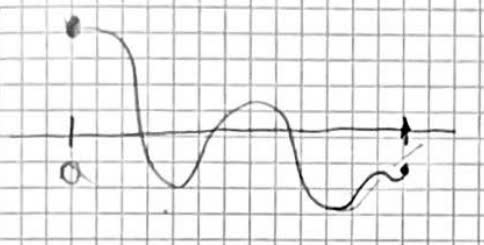
\includegraphics[width=7cm]{images/Screenshot from 2022-09-20 22-39-38.png} }}%
        \qquad
        \subfloat[][\centering The function is taking values at opposite sign at endpoints, which means that the function $f$ has at least one zero in the interval]{{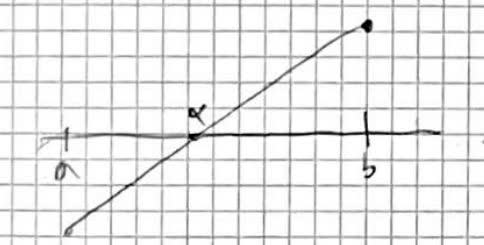
\includegraphics[width=7cm]{images/Screenshot from 2022-09-20 22-39-42.png} }}%
        \captionsetup{justification=centering}
    \end{figure}
\end{enumerate}

Starting from an interval, we shrink it:
$$
\alpha\in I^{(0)}=[a,b]$$
$$
\alpha\in I^{(1)}\subset I^{(0)}$$
$$
|I^{(0)}|=\frac{|I^{(0)}|}{2}$$
$$
\alpha\in I^{(2)}\subset I^{(1)}$$
$$
|I^{(2)}|=\frac{|I^{(1)}|}{2}$$
$$
\vdots
$$

Collection of intervals that are getting smaller and smaller, that all contain $\alpha$ (the zero), so at the end we will get to $\alpha$

Strength point of bisection: \textbf{always convergent, but has a lot of drawbacks too}.

But we are looking for $x^{(k)}$ that approximates $\alpha$
$$?\,\,x^{(k)}\simeq\alpha$$
To do this we consider the midpoint of the interval

\begin{figure}[!ht]
    \begin{minipage}{\linewidth}
        \centering
        \makebox[\textwidth][c]{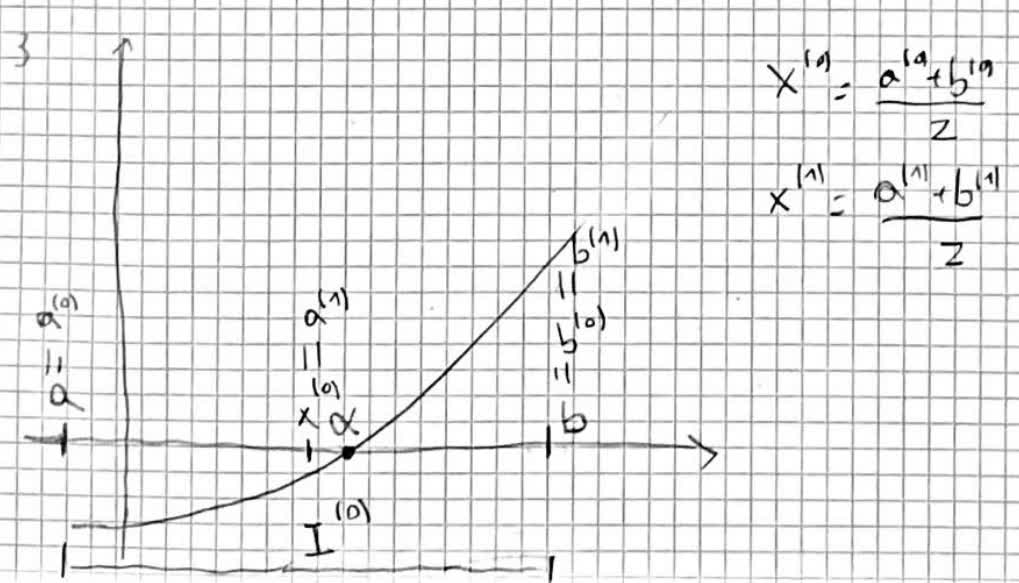
\includegraphics[width=0.8\textwidth]{images/Screenshot from 2022-09-20 22-39-51.png}}%
        %\caption{Function 3}
        %\label{BarsNielsenCrop}
    \end{minipage}
\end{figure}

We see that in this example the first midpoint is already close to $\alpha$. Now we have to choose a new subinterval $I^{(1)}$, we will choose the right subinterval as we need to satisfy the hypothesis that the extremes have opposite signs. We then continue iteratively.

The algorithm is similar to binary search. Formally:\\
\textbf{Inputs}: $a=a^{(0)},\,\,b^{(0)}=v,\,\,f;\,\,TOL,\,\,Nmax$\\
Where $TOL$ is the tolerance and $Nmax$ the maximum number of iterations.

\begin{center}
    \begin{lstlisting}[escapeinside=`']
        while(true)
            `$x^{(k)}=(a^{(k)}+b^{(k)})/2$'
            if(`$f(x^{(k-1)})=0$') break;
            if `$f(a^{(k-1)})f(x^{(k-1)})<0$'
                `$a^{(k)}=a^{(k-1)},b^{(k)}=x^{(k-1)}$';
            else
                `$a^{(k)}=x^{(k-1)},b^{(k)}=b^{(k-1)}$';
            end
        \end{lstlisting}
\end{center}

Regarding the intervals, we see that:
$$
|I^{(k)}|=\frac{b-a}{2^k}=\frac{|I^{(0)}|}{2^k}
$$
$$
|e^{(k)}|=|\alpha-x^{(k)}|<\frac{|I^{(k)}|}{2}=\frac{b-a}{2^{k+1}}
$$
$$
\lim_{k\rightarrow\infty}|e^{(k)}|=(b-a)\lim_{k\rightarrow\infty}\left(\frac{1}{2}\right)^{(k+1)}=0
$$
Regarding the tolerance
$$
?\,\,k\text{ s.t. }|e^{(k)}|\leq TOL=10^{-9}
$$
$$
\frac{b-a}{2^{(k+1)}}\leq TOL
$$
$$
\frac{b-a}{TOL}\leq 2^{(k+1)}
$$
$$
\log_2\left(
    \frac{b-a}{TOL}
\right)\leq k+1
$$
$$
k\geq\log_2\left(
    \frac{b-a}{TOL}
\right)-1
$$
The right member will represent the $Nmax$
$$
Nmax=\left\lceil\log_2\left(
    \frac{b-a}{TOL}
\right)\right\rceil=
\left\lceil\log_{10}\left(
    \frac{b-a}{TOL}
\right)/\log_{10}2\right\rceil
$$

\subsubsection{Pros and Cons}
Pros:
\begin{itemize}
    \item Converges
    \item Can compute maximum number of iterations
\end{itemize}
Cons:
\begin{itemize}
    \item We are losing the monotonicity of the method, a subsequent guess is not guaranteed to find a $x$ closer to $\alpha$ w.r.t. the previous $x$, \textbf{not monotonic w.r.t. to error, the error does not necessarily decreases at each step, we have no convergence order}
    \item Cannot find $\alpha$ in a single step
    \item We are only exploiting the fact that the function is changing sign, function values of $f$ are ignored
\end{itemize}

\subsection{Newton method}
$Nmax$ has to hold for all continuous functions in that interval $[a,b]$, so it has to be large.

The Newton we are not only exploiting the sign of f, but also the values. It is the most powerful method, and demands that:
$$f\in C^1([0,0])$$
Set of functions continuous in their first derivative

Replace $f$ with the tangent line at point of oure initial guess $x^{(0)}$, then take the intersection of the tangent with the $x$ axis, that will be our $x^{(1)}$. Then repeat:

\begin{figure}[!ht]
    \begin{minipage}{\linewidth}
        \centering
        \makebox[\textwidth][c]{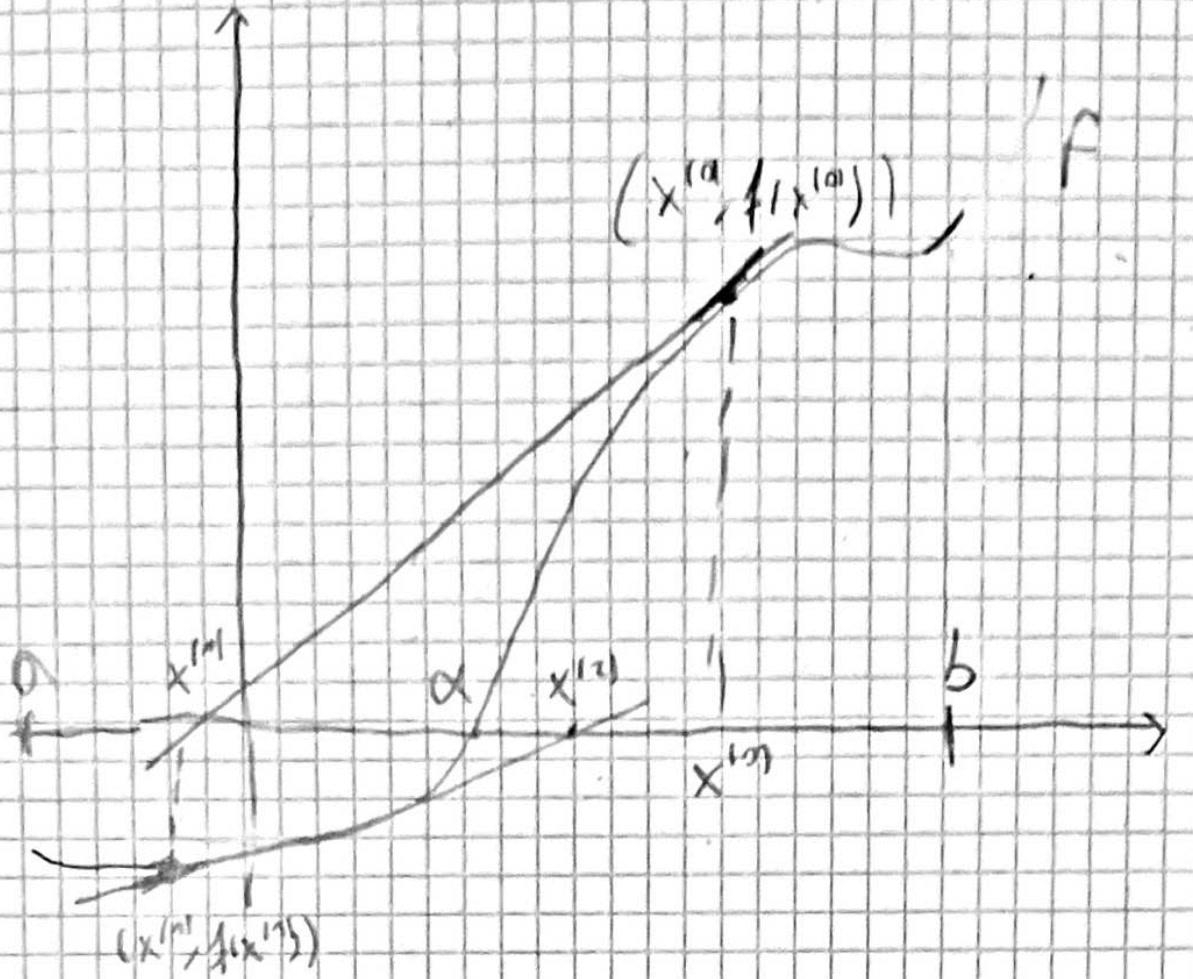
\includegraphics[width=0.8\textwidth]{images/Screenshot from 2022-09-20 22-40-09.png}}%
        %\caption{Tangent Newton method}
        %\label{BarsNielsenCrop}
    \end{minipage}
\end{figure}
tg to $f$ at $(x^{(k)},f(x^{(k)}))\\
y(x)=f(x^{(k)})+f'(x^{(k)})(x-x^{(k)})\\
x^{(k+1)}\text{ s.t. }y(x^{(k+1)})=0\\
f(x^{(k)})+f'(x^{(k)})(x^{(k+1)}-x^{(k)})
$\\
From this equality we want to derive $x^{(k+1)}$:\\
$$x^{(k+1)}=x^{(k)}-\frac{f(x^{(k)})}{f'(x^{(k)})}\qquad k\geq 0$$
Assuming $f'(x^{(k)})\neq 0$\\
It can be proved that this algorithm is just a truncation of the Taylor expansion
\subsubsection{Taylor expansion}
We must first decide the center and where to evaluate the expansion. In oure case the center is $x^{(k)}$, we evaluate at $x^{(k+1)}$
$$f(x)=f(x^{(k)})+f'(x^{(k)})(x-x^{(k)})+O\left((x-x^{(k)})^2\right)x^{(k+1)}$$
So if we evaluate at $x^{(k+1)}$, we simply replace $x$. We neglect the big $O$ term and if $k$ is sufficiently large, we can approximate to $\alpha$.
$$0=f(\alpha)\simeq f(x^{(k+1)})\cong f(x^{(k)})+f'(x^{(k)})(^{(k+1)}-x^{(k)})$$
Which is exactly the Newton method

\subsubsection{Comparison with bisection}
Newton can identify $\alpha$ in a single step.\\
Geometrical proof:

\begin{figure}[!ht]
    \begin{minipage}{\linewidth}
        \centering
        \makebox[\textwidth][c]{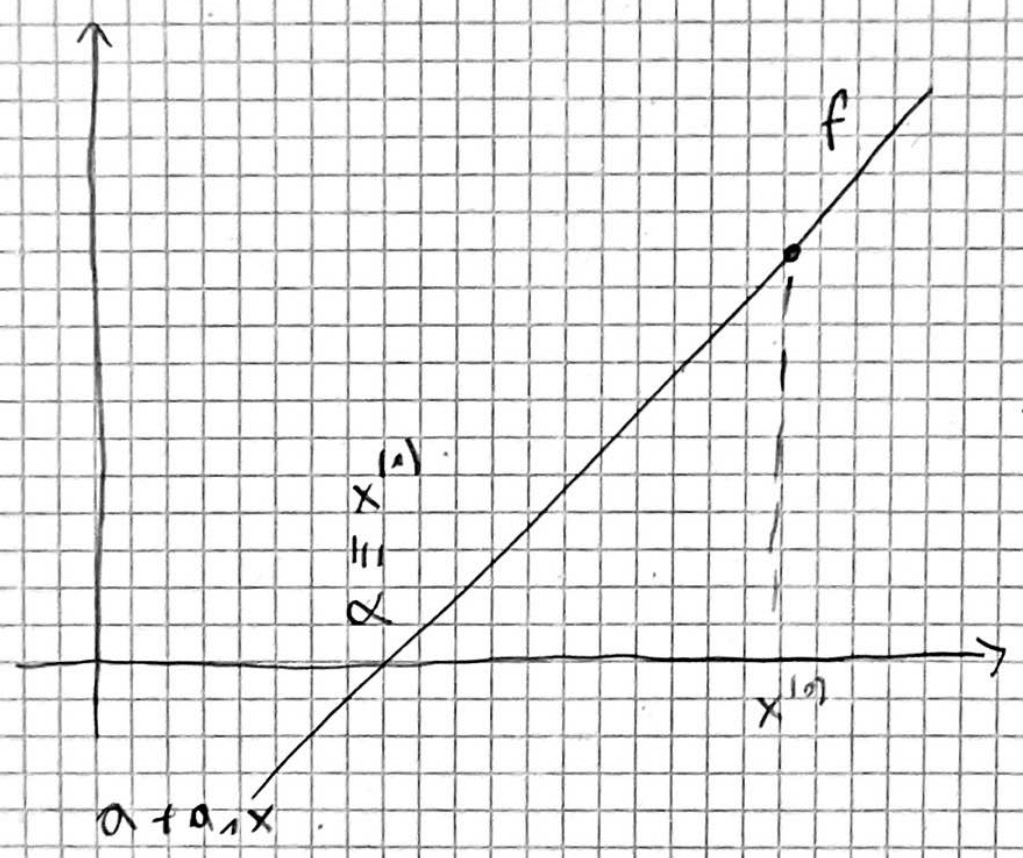
\includegraphics[width=0.5\textwidth]{images/Screenshot from 2022-09-20 22-40-18.png}}%
    \end{minipage}
\end{figure}

Analytical proof:
$$x^{(1)}=x^{(0)}-\frac{f(x^{(0)})}{f'(x^{(0)})}=x^{(0)}-\frac{
    a_0+a_1x^{(0)}
}{a_1}=-\frac{a_0}{a_1}$$

Bisection converges without initial guess, but Newton is better even though it needs an initial guess. \textbf{If initial guess not close to the zero, we do not converge}

\subsubsection{Convergence}
Two hypothesis
\begin{enumerate}[H1)]
    \item $x^{(0)}$ sufficiently close to $\alpha$. But we do not know $\alpha$, we could:
    \begin{itemize}
        \item Graphically plot it
        \item Do some steps of the bisection and use some outputs of it for Newton: \textbf{bisection-Newton: predictor-corrector}, use a weaker method then a stronger one. With bisection we know that we will converge, even if slowly, then after a desired steps (sufficiently close) we use Newton which is faster
    \end{itemize}
    \item $\alpha$ is a simple zero of $f$
    $$
    \begin{cases}
        f(\alpha)=0\\
        f'(\alpha)\neq 0
    \end{cases}
    $$
    Reminder, an $\alpha$ is a zero of order $m$ if
    $$
    \begin{cases}
        f(\alpha)=f'(\alpha)=f''(\alpha)=\cdots=f^{(m-1)}(\alpha)=0\\
        f^{(m)}(\alpha)\neq 0        
    \end{cases}
    $$
\end{enumerate}
$\mathbf{\Rightarrow}$ \textbf{Newton is convergent}

Adding a third hypothesis
\begin{enumerate}[H3)]
    \item $f\in C^2([a,b])$, we can say that the following limit holds:
    $$\lim_{k\rightarrow\infty}\frac{
        x^{(k+1)}\alpha
    }{[x^{(k)}-\alpha]^2}=
    \underlabel{\frac{f''(\alpha)}{2f'(\alpha)}}{C}$$
    In general \textbf{convergence order} equal to P if $\exists\,\,c$ independent from $k$, such that
    $$\frac{|x^{k+1}-\alpha|}{|x^k-\alpha|^P}\leq C,\,\,\forall\,\,k\geq k_0$$
    If $P=1$, linear convergence. In our case $P=2$, quadratic convergence. In general, with a higher convergence order the error reduces:
    
    $
    x^{(k)}-\alpha=10^{-2}\\
    x^{(k)}-\alpha\simeq 10^{-4}\qquad P=2\\
    x^{(k)}-\alpha\simeq 10^{-6}\qquad P=3
    $

    The constant $C$ does not have any requirement, but in some sense it is slowing the convergence (for $C=10,P=3,\text{the error }\simeq 10^{-6}*10=10^{-5}$), but for $P=1$ reduction of the error not guaranteed if $C=1$, so:
    $$P=1\rightarrow C<1$$
    In the Newton case:
    $$C=\frac{f''(\alpha)}{2f'(\alpha)}$$
\end{enumerate}
\subsubsection{Modified Newton scheme}
What if H2 does not hold, can we still use Newton? Yes, but we lose the quadratic order of the convergence.\\
If $\alpha$ is a multiple zero of $f$ (multiplicity $m$) and if $x^{(0)}$ is sufficiently close to $\alpha\Rightarrow$ Newton converges linearly ($P=1$, we lost an order of convergence)

We can use the modified Newton scheme:
$$x^{(k+1)}=x^{(k)}-m\frac{f(x^{(k)})}{f'(x^{(k)})}\qquad k\geq 0$$
Example:
$$f(x)=(x-1)\log(x)$$
$$\alpha=1$$
$$m=2$$
\begin{figure}[!ht]
    \begin{minipage}{\linewidth}
        \centering
        \makebox[\textwidth][c]{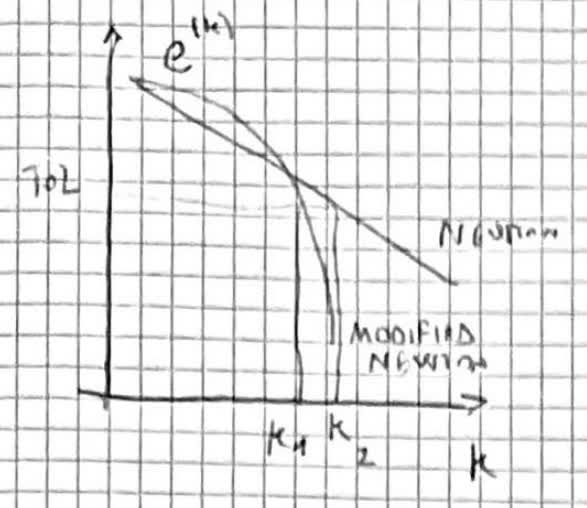
\includegraphics[width=0.6\textwidth]{images/Screenshot from 2022-09-27 18-43-43.png}}%
        %\caption{Modified Newton graph}
        %\label{BarsNielsenCrop}
    \end{minipage}
\end{figure}

\subsubsection{System of nonlinear equations, vector}
$$
\begin{cases}
    f_1(x_1,x_2,\cdots,x_n)=0\\
    f_2(x_1,x_2,\cdots,x_n)=0\\
    \vdots\\
    f_n(x_1,x_2,\cdots,x_n)=0\\
\end{cases}
$$
Example
$$
\begin{cases}
    f_1(x_1,x_2)=x_1^3+\sin x_2=0\\
    f_2(x_1,x_2)=-x_1\sqrt{x_2}+\text{tg}\left(\frac{x_2}{3x_1}\right)=0
\end{cases}
$$
We can rewrite this complex model to a more manageable form, a \textbf{vectorial way}
$$\overrightarrow{x}=[x_1,x_2,\cdots,x_n]^T$$
$$\overrightarrow{f}=[f_1(\overrightarrow{x}),f_2(\overrightarrow{x}),\cdots,f_n(\overrightarrow{x})]^T$$
$$\overrightarrow{0}=[0,\cdots,0]^T\in\mathbb{R}^n$$
So we can rewrite the system of nonlinear equations in:
$$\overrightarrow{f}(\overrightarrow{x})=\overrightarrow{0}$$
Now applying the Newton method, we jsut introduce the vectors that contain the $k$-approximation error:
$$x^{(k+1)}=x^{(k)}-\frac{f(x^{(k)})}{f'(x^{(k)})}$$
Now with
$$\overrightarrow{x}^{(k)}=\left[x_1^{(k)},x_2^{(k)},\cdots,x_n^{(k)}\right]^T\in\mathbb{R}^n$$
$$\overrightarrow{x}^{(k+1)}=\left[x_1^{(k+1)},x_2^{(k+1)},\cdots,x_n^{(k+1)}\right]^T\in\mathbb{R}^n$$
$$\overrightarrow{f}(\overrightarrow{x}^{(k)})=\left[f_1(\overrightarrow{x}^{(k)}),f_2(\overrightarrow{x}^{(k)}),\cdots,f_n(\overrightarrow{x}^{(k)})\right]^T\in\mathbb{R}^n$$
What about the derivative? Use Jacobian
$$x^{(k+1)}=x^{(k)}-\underlabel{\frac{f(x^{(k)})}{f'(x^{(k)})}}{$\delta x^{(k)}$}$$
$$f'(x^{(k)})\delta x^{(k)}=-f(x^{(k)})$$
$$\overrightarrow{x}^{(k+1)}=\overrightarrow{x}^{(k)}+\delta\overrightarrow{x}^{(k)}$$
$$?\,\,\delta\overrightarrow{x}^{(k)}=-\overrightarrow{f}(\overrightarrow{x}^{(k)})$$
The Jacobian
$$\left(J_F\right)_y=\frac{\partial f_i}{\partial x_j}\qquad i,j=1,\cdots,n$$
The question mark becomes
$$
\underlabel{J_F\left(\overrightarrow{x}^{(k)}\right)}{$\mathbb{R}^{n\times n}$}
\underlabel{\delta x^{(k)}}{$\mathbb{R}^n$}=
\underlabel{-\overrightarrow{f}(\overrightarrow{x})^{(k)}}{$\mathbb{R}^n$}
$$

\subsubsection{Bisection - Newton method}
They are predictor-corrector mtehods. Newton is conditional convergent (the initial guess bust be close to the root), while bisection is unconditional convergent: \textbf{by using bisection we are sure that the intial guess is close to the root (predictor) then use Newton as corrector}.

\subsection{Convergence order}

$$
\brackets{x^{(k)}}\simeq\alpha
$$
Convergence order equal to p if $\exists\,\,c$ independent from $k$, such that $\frac{|x^{k+1}-\alpha|}{|x^k-\alpha|^p}\leq c,\,\,\forall\,\,k\geq k_0$
\begin{itemize}
    \item \textbf{Bisection}, error no monotone, no convergence order
    \item \textbf{Newton}
    $$x^{(k+1)}=x^{(k)}-\frac{f(x^{(k)})}{f'(x^{(k)})}\qquad k\geq 0$$
    In Newton, under assumptions that:
    \begin{itemize}
        \item $f(\alpha)=0$
        \item $f'(\alpha)\neq 0$
    \end{itemize}
    $\alpha$ simple zero, we have
    \begin{itemize}
        \item Convergence order of 1 if $f\in C^1$
        \item Convergence order of 2 if $f\in C^2$
    \end{itemize}
    If $\alpha$ not simple, $f\in C^2$, $\alpha$ is a zero of order $m\,\,(f(\alpha)=0,\cdots,f^{(m-1)}(\alpha)=0,f^{(m)}(\alpha)\neq 0)$, more simply when there is a power the zero is of the order of that power.
    \item \textbf{Modified Newton method}, unlike bisection, with newton we can compute the convergence order. Can find non-simple zeros, we have a convergence order of 2 for example. We use a different update rule:
    $$x^{(k+1)}=x^{(k)}-m\frac{f(x^{(k)})}{f'(x^{(k)})}\qquad k\geq 0$$
\end{itemize}
$$e=\brackets{|x^k-\alpha|}_k$$
$$e^k=|x^k-\alpha|$$
$$\text{Convergence order = }p=\frac{
\log\left[
    \frac{e^{k+2}}{e^{k+1}}
\right]
}{
\log\left[
    \frac{e^{k+1}}{e^{k}}
\right]
}$$
\textbf{Do not mix up exponential and error, the $e^{k}$ there stands for the error vector considering index from $k$ to $end$}

\subsection{Stopping criteria/point}
$$\underlabel{|x^{(k)}-\alpha|}{$e^{(k)}$}\leq \underlabel{CS}{Error estimator}<TOL$$
$$
\left|e^{(kmin)}\right|=\left|x^{(kmin)}-\alpha\right|\leq CS=C\left|x^{(kmin+1)}-x^{(kmin)}\right|\leq TOL\,\,(e.g.=10^{-9})
$$
A constant that multiplies our error estimator $S$. If large like $10^4$ we lose 4 orders. It is called the \textbf{reliability}, if
\begin{itemize}
    \item $C=O(1)$, estimator reliable
    \item $C=O(10^s)$, not reliable
\end{itemize}
Two kinds of estimators for the error, when one not reliable, can rely on the other one
$$
S=
\begin{cases}
    x^{(k+1)}-x^{(k)}\text{ increment, if convergence this difference becomes smaller and smaller}\\
    \qquad\text{\textbf{Newton}}\\
    r^{(k)}=f(x^{(k)})\text{ residual, huge if $x^{(k)}$ far from $\alpha$, less it is, smaller is the error}\\
    \qquad\text{\textbf{Bisection}}
\end{cases}
$$

The increment one, cycle till:
$$|x^{(k+1)}-x^{(k)}|>TOL\,\,\&\&\,\,i<TOL$$

\pagebreak

\subsubsection{Reliability of the residual}
\begin{figure}[!ht]
    \begin{minipage}{\linewidth}
        \centering
        \makebox[\textwidth][c]{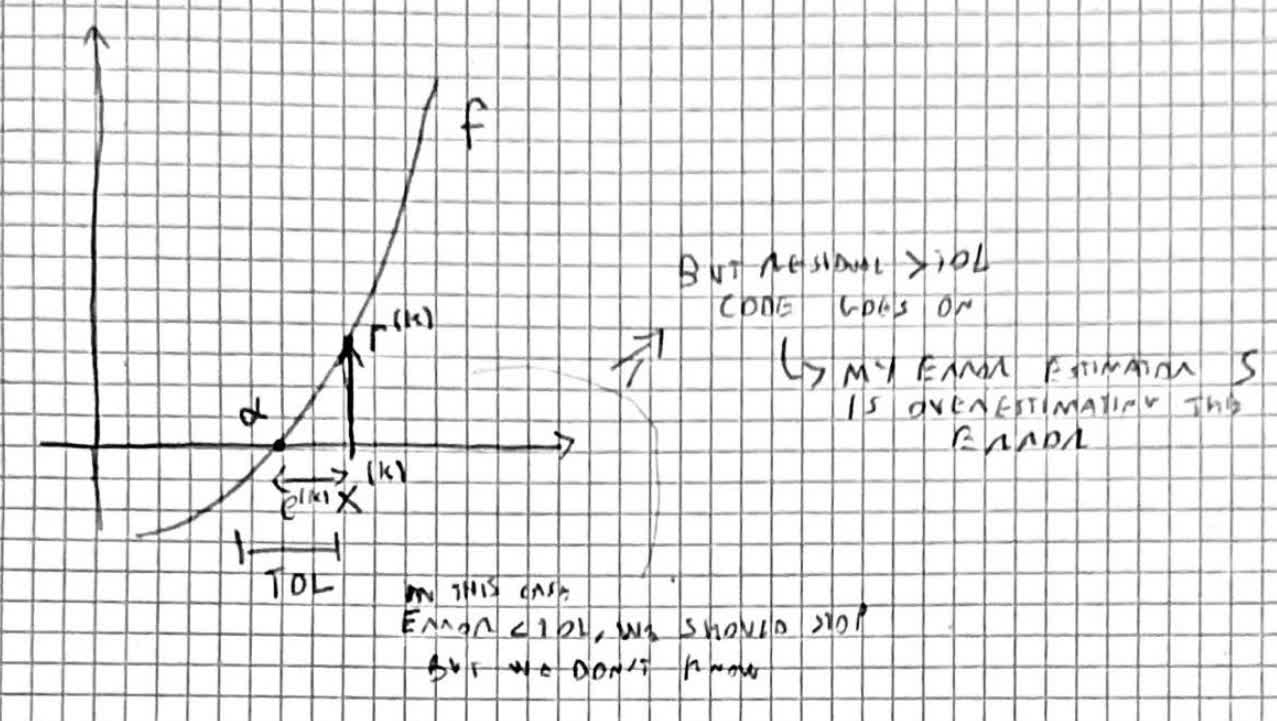
\includegraphics[width=1\textwidth]{images/Screenshot from 2022-09-27 18-43-57.png}}%
        \caption{Overestimating}
        %\label{BarsNielsenCrop}
    \end{minipage}
\end{figure}
My error estimator $S$ is overestimating the error $e^{(k)}$
$$|f'(\alpha)| >> 1$$

\begin{figure}[!ht]
    \begin{minipage}{\linewidth}
        \centering
        \makebox[\textwidth][c]{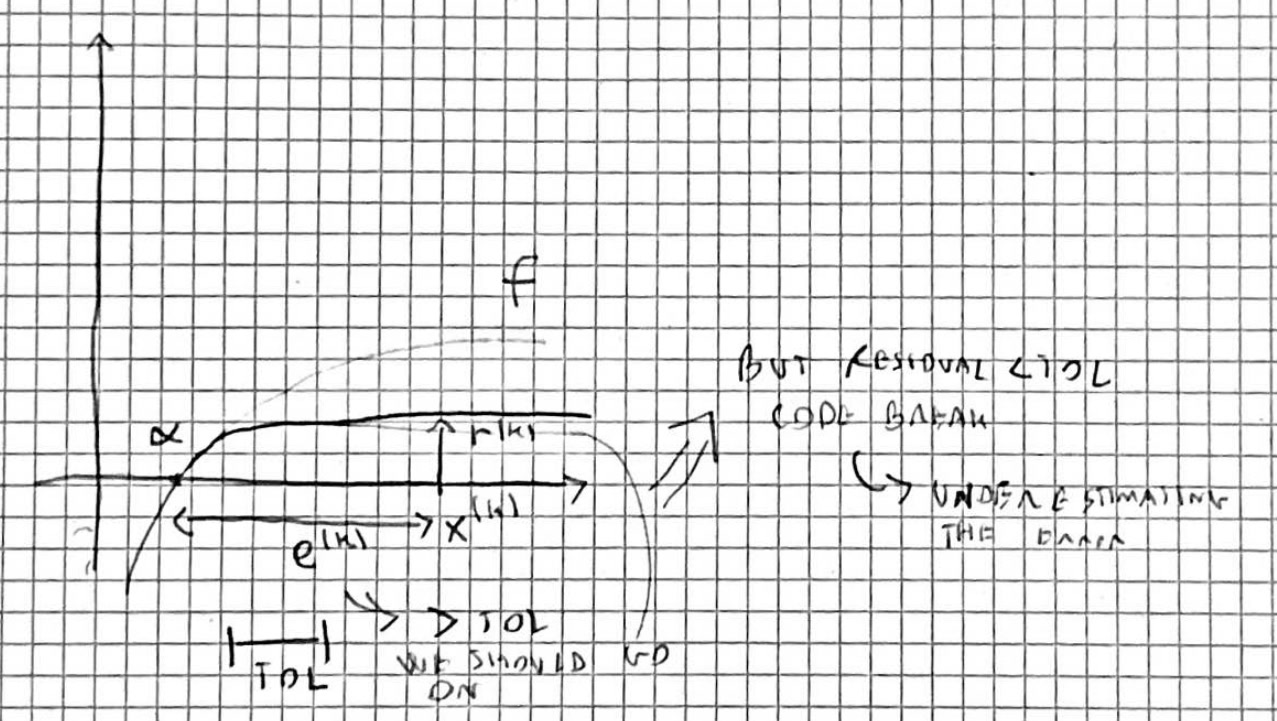
\includegraphics[width=1\textwidth]{images/Screenshot from 2022-09-27 18-44-12.png}}%
        \caption{Underestimating}
        %\label{BarsNielsenCrop}
    \end{minipage}
\end{figure}
My error estimator $S$ is underestimating the error $e^{(k)}$
$$|f'(\alpha)| << 1$$

What's better? Better when overestimating, we do a little more work, but at the end we get the better result

So this estimator is reliable when:
$$|f'(\alpha)| \simeq 1$$

\subsection{Fixed Point Method}
If we apply continuously for example the cos:

$
x^{(0)}=1\\
x^{(1)}=\cos(x^{(0)})\\
x^{(2)}=\cos(x^{(1)})\\
\vdots\\
x^{(k+1)}=\cos(x^{(k)})
$

Which means $\alpha=\cos(\alpha)$, with $\alpha$ known as \textbf{fixed point} of the function cos. In general:
$$\Phi:[a,b]\subset\mathbb{R}\rightarrow \mathbb{R}$$
$$\alpha\in\mathbb{R}\text{ fixed point $\phi(\alpha)=\alpha$}$$
Geometrically we are looking for the intersection of:
$$
\begin{cases}
    y=\phi(x)\\
    y=x\qquad\text{Bisector line}
\end{cases}
$$

\begin{figure}[!ht]
    \begin{minipage}{\linewidth}
        \centering
        \makebox[\textwidth][c]{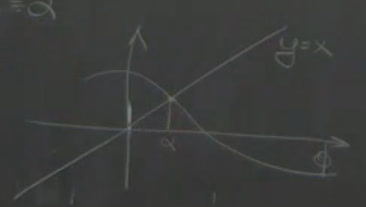
\includegraphics[width=0.8\textwidth]{images/Screenshot from 2022-10-02 16-20-18.png}}%
        %\caption{Fixed point geometric interpretation}
        %\label{BarsNielsenCrop}
    \end{minipage}
\end{figure}

\begin{itemize}
    \item Does any function has a fixed point? No, for example parallel line or exponential function, it grows fast and does not encounter the bisector line
    \item Does a function admit more fixed points? Yes, function can encounter the bisector line multiple times
\end{itemize}
How can a fixed point interest us? We can talk about a sort of duality problem:
$$
\begin{cases}
    ?\,\,\alpha\in\mathbb{R}\,\,st\,\,f(\alpha)=0\qquad\text{Our original problem of zeros}\\
    ?\,\,\alpha\in\mathbb{R}\,\,st\,\,\phi(\alpha)=\alpha\qquad\text{Fixed point problem}
\end{cases}
$$

\subsubsection{Problems correlation}
The transition:
$$
\begin{bmatrix}
    ?\,\,\alpha\in\mathbb{R}\,\,st\,\,f(\alpha)=0 & \Leftrightarrow & ?\,\,\alpha\in\mathbb{R}\,\,st\,\,\phi(\alpha)=\alpha\\
    \\
    f(x)=0 & \Leftrightarrow & \underlabel{f(x)+x}{$\phi(x)$}=x
    \\
    \\
    \Rightarrow \text{Hp: }f(\alpha)=0 & &\Leftarrow\text{Hp: }\phi(\alpha)=\alpha\\
    \text{Th: }\phi(\alpha)=\alpha & & \text{Th: }f(\alpha)=0\\
    \phi(\alpha)=\underlabel{f(\alpha)}{=0}+\alpha=\alpha & & \underlabel{\phi(\alpha)}{$=\alpha$}=f(\alpha)+\alpha=\alpha
\end{bmatrix}
$$
But the $\phi$ is not unique, we can build more and different fixed point functions (e.g. add constant multiplier), this is a \textbf{advantage}, we can pick a function that is for sure to have a fixed point

\subsubsection{The method with Newton and Bisection}
With an \textbf{iterative process}, now we try to solve
$$?\,\,\alpha\in\mathbb{R}\,\,st\,\,\phi(\alpha)=\alpha$$
With iterative method
$$x^{(k+1)}=\phi(x^{(k)})\qquad k\geq 0$$
With initial guess $x^{(0)}$. Considering the previous methods bisection and Newton, can we rewrite them as a fixed point method?
\begin{itemize}
    \item \textbf{Newton}: we can just pick a fixed point function as:
    $$\phi_N(x)=x-\frac{f(x)}{f'(x)}$$
    \item \textbf{Bisection}: no, the midpoint depends on two variables, so bisection is not an example of fixed point method
\end{itemize}

\pagebreak
\subsubsection{Convergence}
\begin{figure}[!ht]
    \begin{minipage}{\linewidth}
        \centering
        \makebox[\textwidth][c]{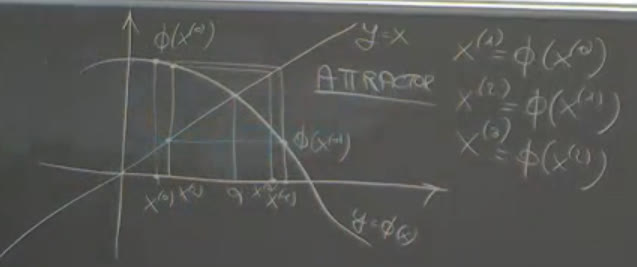
\includegraphics[width=0.8\textwidth]{images/Screenshot from 2022-10-02 17-20-18.png}}%
        \caption{Attractor}
        %\label{BarsNielsenCrop}
    \end{minipage}
\end{figure}

All even at left side, all even at right side.\\
Are we converging to $\alpha$? Yes, the iterations are moving closer and closer to $\alpha$, which is an \textbf{attractor}.

\begin{figure}[!ht]
    \begin{minipage}{\linewidth}
        \centering
        \makebox[\textwidth][c]{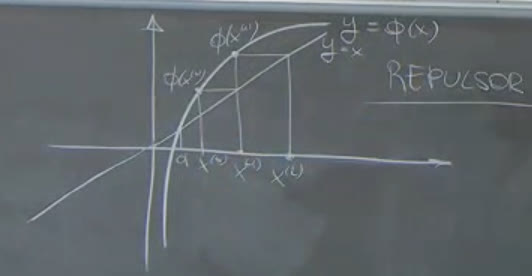
\includegraphics[width=0.8\textwidth]{images/Screenshot from 2022-10-02 17-20-20.png}}%
        \caption{Repulsor}
        %\label{BarsNielsenCrop}
    \end{minipage}
\end{figure}

In this case we are unlucky, we diverge, \textbf{repulsor}.

These are two particular cases, in total there are four: left-right convergent, left-right divergent, one direction convergent, one direction divergent.

Can we identify some features that are responsible for the convergent and divergent trend? The \textbf{value of the derivative $\phi'(\alpha)$ if less or greater than 1}

\pagebreak
\subsubsection{Global and Local Convergence Results}
$$x^{(k+1)}=\phi(x^{(k)})$$
\begin{itemize}
    \item \textbf{Global result}
    \begin{enumerate}
        \item Let $\phi\in C^0([a,b])$ and s.t. $\phi\in[a,b]\,\,\forall\,\,x\in[a,b]$\\
        \begin{figure}[!ht]
            \begin{minipage}{\linewidth}
                \centering
                \makebox[\textwidth][c]{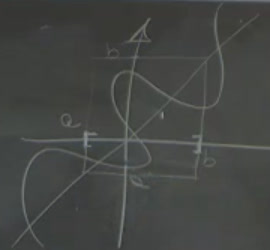
\includegraphics[width=0.4\textwidth]{images/Screenshot from 2022-10-02 17-28-19.png}}%
                %\caption{Demand 1}
                %\label{BarsNielsenCrop}
            \end{minipage}
        \end{figure}
        
        We are demading that our function $\phi$ has to take values inside that rectangle, must be limited in a certain portion of the plane.\\
        Under this hypothesis, we can prove that exists at least a fixed point $\alpha\in\,\,[a,b]$ for function $\phi$ (the example has two), so \textbf{not uniqueness of fixed point}
        \item If we in addition we assume that there exists and integer $L<1$ s.t.
        $$\left|\phi(x_1)-\phi(x_2)\right|\leq L|x_1-x_2|\,\,\forall\,\,x_1,x_2\in[a,b]$$
        (Lipschitz continuity, weaker demand w.r.t. derivability, weaker than $C^1$) then $\exists!\,\,\alpha\in[a,b]$ for $\phi$ and
        $$\brackets{x^{(k)}}\rightarrow\alpha\,\,\forall\,\,x^{(0)}\in\mathbb{R}$$
        Collection of approximations, with this assumption we get \textbf{uniqueness of fixed point and convergence of method independently from initial guess}.\\
        About the \textbf{rate of convergence of fixed point scheme with Lipschitz}, consider the error associated with $k+1$:
        $$|x^{(k+1)}-\alpha|=|\phi(x^{(k)})-\phi(\alpha)|\leq L|x^{(k)}-\alpha|$$
        $$\frac{|x^{(k+1)}-\alpha|}{|x^{(k)}-\alpha|}\leq L < 1$$
        Which means that the fixed method is convergent with order 1 (power below is 1, but actually $p\geq 1$, so \textbf{order at least 1})
    \end{enumerate}
    But this practical is not practical
    \item \textbf{Local result or Ostrowski's theorem}: let $\alpha$ be a fixed point for $\phi$ in $[a,b]$ (so we are already assuming the existence and uniqueness of $\alpha$), with $\phi\in C^1(I_\alpha)$ and $I_\alpha$ neighborhood of $\alpha$ (different from before, we here stronger assumptions than global which only required $C^0$ and Lipschitz continuity, but $C^1$ locally).\\
    Under these hypotheses, if $|\phi'(\alpha)|<1$ then $\exists\,\,\delta>0$ s.t. $\forall\,\,x^{(0)}$ with $|x^{(0)}-\alpha|<\delta$:
    $$\brackets{x^{(k)}}\rightarrow\alpha \text{ and }\lim_{k\rightarrow\infty}\frac{x^{(k+1)}-\alpha}{x^{(k)}-\alpha}=\phi'(\alpha)$$
    To summarize if:
    $$
    \begin{cases}
        |\phi'(\alpha)| < 1 \text{ convergence}\\
        |\phi'(\alpha)| > 1 \text{ divergence}\\
        |\phi'(\alpha)| = 1 \text{ we cannot say anything}\\
    \end{cases}
    $$
\end{itemize}

\subsubsection{Examples for the Local Result}
\begin{enumerate}
    \item $\phi(x)=\cos(x)$ and $\phi'(x)=-\sin(x)$
    $$|\phi'(\alpha)|=|\sin(\alpha)|<1\qquad \alpha\neq 0$$
    \item $\phi(x)=x^2-1$, we want to know if fixed point method is convergent or not: first we derive the fixed point of $\phi$:
    $$x=\phi(x)\rightarrow x^2-x-1=0$$
    $$\alpha_{1,2}=\frac{1\pm\sqrt{5}}{2}$$
    So two fixed point, now compute derivative
    $$\phi'(x)=2x\rightarrow|\phi'(\alpha)|=\left|1\pm\sqrt{5}\right|$$
    In neither cases the module is less than 1, so divergent fixed point method
    \item $\log(x)=\gamma$ with $\gamma\in\mathbb{R}$, we are demanded to approximate this function with fixed point:
    $$f(x)=0\rightarrow \underlabel{\log(x)-\gamma}{$f(x)$}=0$$
    We can use whatever method/fixed point function we like:
    \begin{enumerate}
        \item With Newton
        $$\phi_1(x)=\phi_N(x)=x-\frac{\log(x)-\gamma}{\frac{1}{x}}=x(1-\log(x)+\gamma)$$
        \item 
        $$\phi_2(x)=\log(x)-\gamma+x$$
        \item 
        $$x\log(x)-\gamma x=0\rightarrow\phi_3(x)=\frac{x\log(x)}{\gamma}$$
    \end{enumerate}
    For $\gamma=-2$, we can verify that $\phi_1$ and $\phi_3$ are ok, while for the $\phi_2$ it does not work
\end{enumerate}

\subsubsection{Fixed point method with any order of convergence}
Proposition: let us assume that the Ostrowski's theorem hypothesis are verified (\textbf{so we are in local setting}). If $\phi\in C^P(I_\alpha)$ and $\phi^{(i)}(\alpha)=0\,\,i=1,\cdots,p-1$ (derivatives till $p-1$) and $\phi^{(p)}(\alpha)\neq 0$ then $\exists\,\,\delta>0$ s.t. $\forall\,\,x^{(0)}$ with $\left|x^{(0)}-\alpha\right|<\delta$
$$
\brackets{x^{(k)}}\rightarrow\alpha\text{ and }\lim_{k\rightarrow\infty}\frac{x^{(k+1)}-\alpha}{\left[x^{(k)}-\alpha\right]^p}=\underlabel{\frac{\phi^{(p)}}{p!}}{$C$}
$$
We can guarantee the convergence of our fixed point method and compute the convergence order.

\subsubsection{Stopping criteria}
Reminder
$$
\left|e^{(kmin)}\right|=\left|x^{(kmin)}-\alpha\right|\leq CS=\left|x^{(kmin+1)}-x^{(kmin)}\right|\leq TOL\,\,(e.g.=10^{-9})
$$
Reminder: $\exists\,\,\beta_k$ between $\alpha$ and $x^{(k)}$ (min value theorem, appliable since $\phi$ is $C^1$)
$$
\alpha-x^{(k+1)}=\phi(\alpha)-\phi(x^{(k)})=\phi'(\beta_k)(\alpha-x^{(k)})
$$
So, adding and subtracting $x^{(k+1)}$:
$$
\alpha-x^{(k)}=\alpha-x^{(k+1)}+\underlabel{x^{(k+1)}-x^{(k)}}{$\delta^{(k)}$}=\phi'(\beta_k)(\alpha-x^{(k)})+\delta^{(k)}
$$
$$
\alpha-x^{(k)}=\frac{1}{1-\phi'(\beta_k)}(x^{(k+1)}-x^{(k)})
$$
For $k$ sufficiently large we can identify $x^{(k)}$ with $\alpha$ and $\beta_k$ with $\alpha$. So the error associated with the $k$ iteration is:
$$
\alpha-x^{(k)}\cong\underlabel{\frac{1}{1-\phi'(\alpha)}}{$C$}(x^{(k+1)}-x^{(k)})
$$
For $C$ as much as possible close to 1, it means that $\phi'(\alpha)$ is very small, almost zero.
$$
\phi'(\alpha)=0\rightarrow\text{convergence order of at least 2! Quadratic convergence}
$$

An \textbf{example}:
$$
f(x)=(x-1)^{(n-1)}\log(x)
$$
With one zero $\alpha=1$ with multeplicity $m$. We can prove that:
$$\phi'(\alpha)=1-\frac{1}{m}$$
Larger is $m$, closer that quantity is to 1, which means we are losing in terms of reliability ($C$ is growing to infinity).

\begin{figure}[!ht]
    \begin{minipage}{\linewidth}
        \centering
        \makebox[\textwidth][c]{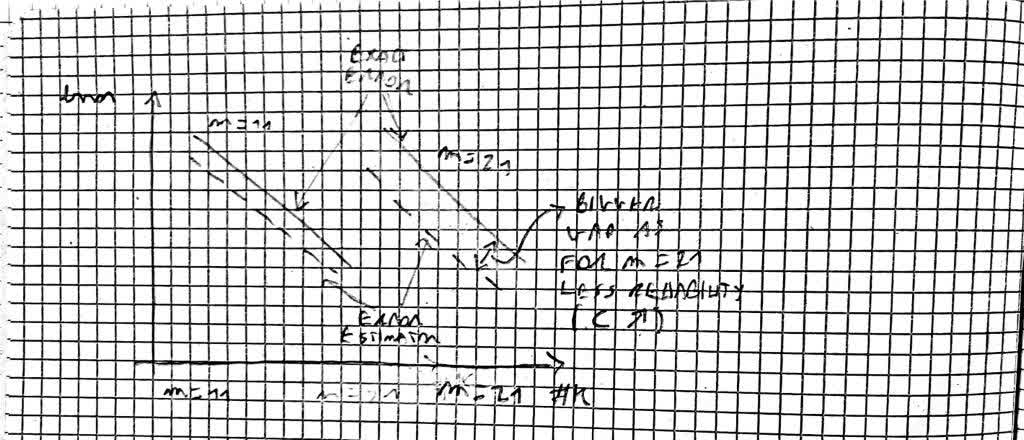
\includegraphics[width=1\textwidth]{images/Screenshot from 2022-10-04 17-28-19.png}}%
        %\caption{Trend of error and error estimator}
        %\label{BarsNielsenCrop}
    \end{minipage}
\end{figure}

A stopping criterion for fixed point: $m$ not too high.

\subsection{Consistency}
$$
x^{(k+1)}=\phi(x^{(k)})
$$
If $\alpha$ is a fixed point of $\phi$, the method is consistent